
\documentclass[14pt]{extbook}
%General Packages
\usepackage{multicol, enumerate, enumitem, hyperref, color, soul, setspace, parskip, fancyhdr}

%Math Packages
\usepackage{amssymb, amsthm, amsmath, bbm, latexsym, units, mathtools}

%All math in Display Style
\everymath{\displaystyle}

% Packages with additional options
%\usepackage[T1]{fontenc}
\usepackage[headsep=0.5cm,headheight=12pt, left=1 in,right= 1 in,top= 1 in,bottom= 1 in]{geometry}
\usepackage[usenames,dvipsnames]{xcolor}

% SageTeX
\usepackage{sagetex}

% Package to use the command below to create lines between items
\usepackage{dashrule}
\newcommand{\litem}[1]{\item#1\hspace*{-1cm}\rule{\textwidth}{0.4pt}}

\pagestyle{fancy}
\lhead{Module\,12L\,-\,Graphing\,Rational\,Functions}
\chead{}
\rhead{Progress Exam 6}
\lfoot{Summer\,C\,2020}
\cfoot{}
\rfoot{Version B}

\begin{document}
\pagestyle{fancy}

\begin{sagesilent}
load("../Code/generalPurposeMethods.sage")
load("../Code/keyGeneration.sage")
load("../Code/commonlyUsedFunctions.sage")
keyFileName = "Module12L"
version = "B"
\end{sagesilent}

\begin{enumerate}
%\setcounter{enumi}{75}


  \begin{sagesilent}
  moduleNumber="12L"
  problemNumber=76
  load("../Code/16graphingRationalFunctions/identifyGraphOfRationalFunction.sage")
  \end{sagesilent}

  \litem{ \sage{displayStem}

   \begin{center}
       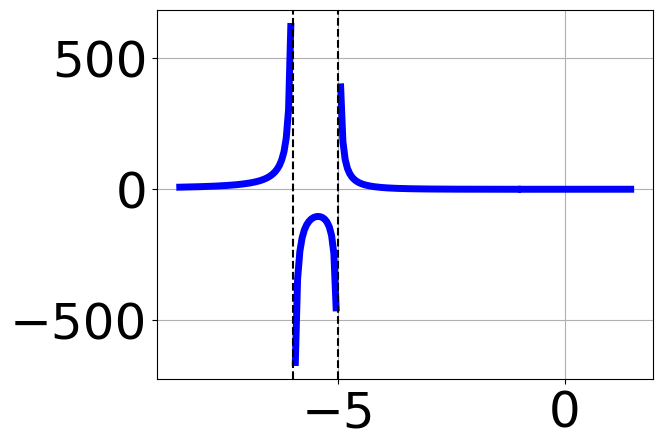
\includegraphics[width=0.5\textwidth]{../Figures/identifyGraphOfRationalFunctionB.png}
   \end{center}

  	\begin{enumerate}[label=\Alph*.]
    \item \( \sage{choices[0]} \)
    \item \( \sage{choices[1]} \)
    \item \( \sage{choices[2]} \)
    \item \( \sage{choices[3]} \)
    \item \( \sage{choices[4]} \)
  	\end{enumerate}
  }
\begin{sagesilent}
moduleNumber="12L"
problemNumber=77
load("../Code/16graphingRationalFunctions/identifyOAs.sage")
\end{sagesilent}

\litem{ \sage{displayStem}

   \[ \sage{displayProblem} \]

  	\begin{enumerate}[label=\Alph*.]
    \item \( \sage{choices[0]} \)
    \item \( \sage{choices[1]} \)
    \item \( \sage{choices[2]} \)
    \item \( \sage{choices[3]} \)
    \item \( \sage{choices[4]} \)
  	\end{enumerate}
  }
\begin{sagesilent}
moduleNumber="12L"
problemNumber=78
load("../Code/16graphingRationalFunctions/identifyVAs.sage")
\end{sagesilent}

\litem{ \sage{displayStem}

   \[ \sage{displayProblem} \]

  	\begin{enumerate}[label=\Alph*.]
    \item \( \sage{choices[0]} \)
    \item \( \sage{choices[1]} \)
    \item \( \sage{choices[2]} \)
    \item \( \sage{choices[3]} \)
    \item \( \sage{choices[4]} \)
  	\end{enumerate}
  }
\begin{sagesilent}
moduleNumber="12L"
problemNumber=79
load("../Code/16graphingRationalFunctions/identifyHAs.sage")
\end{sagesilent}

\litem{ \sage{displayStem}

   \[ \sage{displayProblem} \]

  	\begin{enumerate}[label=\Alph*.]
    \item \( \sage{choices[0]} \)
    \item \( \sage{choices[1]} \)
    \item \( \sage{choices[2]} \)
    \item \( \sage{choices[3]} \)
    \item \( \sage{choices[4]} \)
  	\end{enumerate}
  }
\begin{sagesilent}
moduleNumber="12L"
problemNumber=80
load("../Code/16graphingRationalFunctions/identifyHoles.sage")
\end{sagesilent}

\litem{ \sage{displayStem}

   \[ \sage{displayProblem} \]

  	\begin{enumerate}[label=\Alph*.]
    \item \( \sage{choices[0]} \)
    \item \( \sage{choices[1]} \)
    \item \( \sage{choices[2]} \)
    \item \( \sage{choices[3]} \)
    \item \( \sage{choices[4]} \)
  	\end{enumerate}
  }

\end{enumerate}

\end{document}

